\section{Implicit ODE solver} \label{part3}
We consider again the initial value problem in (\ref{2_problem}).

\subsection{Describe the implicit Euler algorithm (i.e. provide an algorithm for it in
your report and explain how you get from the differential equations to the
numerical formulas).}
The idea behind the Implicit Euler is that, instead of using the function evaluation at the previous point, it uses the one at the future point. A more mathematical derivation would be to approximate the integral form of the problem by the right-hand rectangle method, as in
\begin{equation*}
    x(t_{n+1})- x(t_n) = \int_{t_n}^{t_{n+1}} f(t,x(t),p) dt \approx hf(t+1,x(t+1),p).
\end{equation*}
As seen in part \ref{part1}, this improves the absolute region of stability of the Explicit Euler considerably. However, the bad news is that a nonlinear system of equations must be solved in each time step. To achieve this we'll use Newton's method to approximate the solution. The Implicit Euler is therefore calculated as:
\begin{align*}
    x_0 &= x(t_0), \\
    x_n &= x_{n-1} + hf(t_n, x_n, p), \hspace{1em} \text{solve } x_n \text{ for } n = 1,2,\ldots, N.
\end{align*}

%%%%%%%%%%%%%%%%%%%%%%%%%%%%%%%%%%%%%%%%%%%%%%%%%%%%%%%%%%%%%%%%%%%%%%%%%%%%%%%%%%%%%%%%%%%%%%%%%%%

\subsection{Implement  an  algorithm  in  Matlab  for  the  implicit  Euler  method  with
 fixed time-step and provide this in your report.  Use a format that enables
syntax highlighting.}

\begin{lstlisting}[caption = Newton's method, captionpos=b, label=3_NewtonsMethod]
 function [x,k] = NewtonsMethod(FunJac, tk, xk, h, xinit, tol, maxit, args)
k = 0;
t = tk + h;
x = xinit;
[f,J] = feval(FunJac,t,x,args{:});
k = k + 1;
R = x - h*f - xk;
I = eye(length(xk));

while( (k<maxit) && (norm(R,'inf')>tol) )
    dRdx = I - J*h;
    dx = dRdx\R;
    x = x - dx;
    [f,J] = feval(FunJac,t,x,args{:});
    k = k+1;
    R = x - h*f - xk;
end

\end{lstlisting}
\begin{lstlisting}[caption = Implicit Euler method with fixed time step size, captionpos=b, label=3_ImEuler_fixed]
function [T,X] = EulerImplicit_fixed(funJac, tspan, h, x0, args)

t0 = tspan(1);
tf = tspan(end);
T = t0:h:tf;
N = size(T,2);
X = zeros(size(x0,1), N);
X(:,1) = x0;

tol = 1.0e-8;
maxit = 100;

for k=1:N-1
    f = feval(funJac,T(k),X(:,k),args{:});
    xinit = X(:,k) + f*h;
    [X(:,k+1),~] = NewtonsMethod(funJac, T(:,k), X(:,k), h, xinit, tol, maxit, args);
end
end

\end{lstlisting}
%%%%%%%%%%%%%%%%%%%%%%%%%%%%%%%%%%%%%%%%%%%%%%%%%%%%%%%%%%%%%%%%%%%%%%%%%%%%%%%%%%%%%%%%%%%%%%%%%%%

\subsection{ Implement  an  algorithm  in  Matlab  for  the  implicit  Euler  method  with
adaptive time step and error estimation using step doubling.}
The Implicit Euler with adaptive time step will also call Newton's method shown in Listing \ref{3_NewtonsMethod}
\begin{lstlisting}[caption = Implicit Euler method with fixed time step size, captionpos=b, label=3_ImEuler_adaptive]
function [T,X,r_out,h_out,info] = EulerImplicit_adaptive(funJac,tspan,h0,x0,abstol,reltol,args)

epstol = 0.8;
facmin = 0.1;
facmax = 5.0;

newtontol = 1.0e-8;
maxit = 100;

t0 = tspan(1);
tf = tspan(end);
t = t0;
h = h0;
x = x0;

T = t0;
X = x0;
r_out = [];
h_out = [h0];
info = zeros(1,4);

nfun = 0;
nstep = 0;
naccept = 0;

while t < tf
    if (t+h > tf)
        h = tf-t;
    end
    [f,J] = feval(funJac,t,x,args{:});
    nfun = nfun + 1;
    
    AcceptStep = false;
    while ~AcceptStep
        % Single step size
        xinit1 = x + h*f;
        [x1,nfun_local] = NewtonsMethod(funJac, t, x, h, xinit1, newtontol, maxit, args);
        nfun = nfun + nfun_local;
        
        hm = 0.5*h;
        tm = t + hm;
        xinitm = x + hm*f;
        [xm,nfun_local] = NewtonsMethod(funJac, t, x, hm, xinitm, newtontol, maxit, args);
        nfun = nfun + nfun_local;
        
        [fm,Jm] = feval(funJac,tm,xm,args{:});
        nfun = nfun + 1;
        xinit1hat = xm + hm*f;
        [x1hat,nfun_local] = NewtonsMethod(funJac, tm, xm, hm, xinit1hat, newtontol, maxit, args);
        nfun = nfun + nfun_local;
        
        nstep = nstep + 1;
        
        e = abs(x1hat-x1);
        r = max(e./max(abstol, abs(x1hat) .* reltol));
        AcceptStep = (r <= 1.0);
        
        if AcceptStep
            t = t+h;
            x = x1hat;
            
            T = [T,t];
            X = [X,x];
            r_out = [r_out, r];
            h_out = [h_out, h];
            naccept = naccept + 1;
        end
        
        h = max(facmin, min(sqrt(epstol/r), facmax)) * h;
    end
end

info(1) = nfun;
info(2) = nstep;
info(3) = naccept;
info(4) = nstep - naccept;

end

\end{lstlisting}

%%%%%%%%%%%%%%%%%%%%%%%%%%%%%%%%%%%%%%%%%%%%%%%%%%%%%%%%%%%%%%%%%%%%%%%%%%%%%%%%%%%%%%%%%%%%%%%%%%%

\subsection{Test your algorithms on the Van der Pol problem \texorpdfstring{($\mathbf{\mu = 2}$ and $\mathbf{\mu = 12}$, $\mathbf{x_0 = [0.5;0.5]}$).}{(mu = 2 and mu = 12, x0 = [0.5;0.5]).}}
The way of calling the ODE solvers is similar as in Exercise \ref{2_4}. Results are shown in the following Figures and Tables. First thing we can notice when looking at the plot is that the Implicit, contrary to the Explicit, approximates the error from the inside of the steady-state curve: worst approximations of the solution make the frequency of the oscillation larger and the amplitude smaller.

We can also observe the stiffness of $\mu=12$ is handled a lot better. Specially in Figure \ref{3_4_adaptive_mu_12}, while there's still some oscillations when $x_2$ shifts suddenly, it is considerably better than the Explicit. It's also worth noticing, looking at Tables \ref{3_4_adaptive_mu_2_table} and \ref{3_4_adaptive_mu_12_table}, the huge increase in the number of function evaluations. This is obviously due to the added call to Newton's method to solve the non linear equation.

\begin{figure}[H]
    \centering
    \makebox[\textwidth][c]{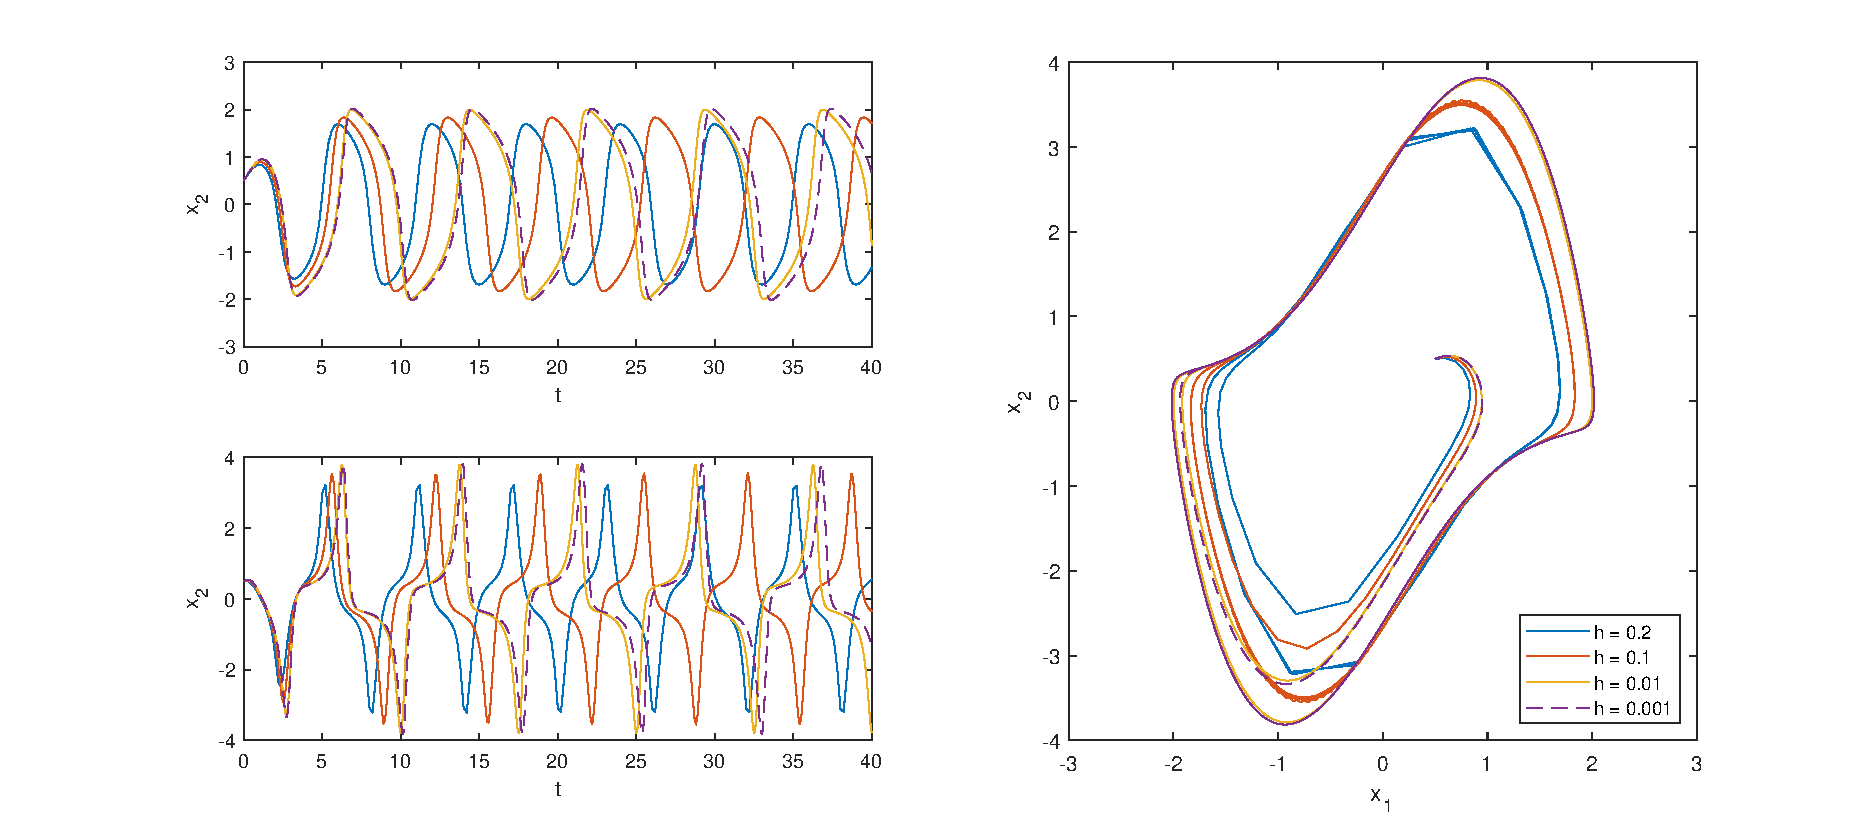
\includegraphics[width=1.25\textwidth]{images/3/3_4_fixed_mu_2.pdf}}
    \caption{Solution for the Van der Pol problem ($\mathit{\mu = 2}$) using Implicit Euler with fixed step size}
    \label{3_4_fixed_mu_2}
\end{figure}

\begin{figure}[H]
    \centering
    \makebox[\textwidth][c]{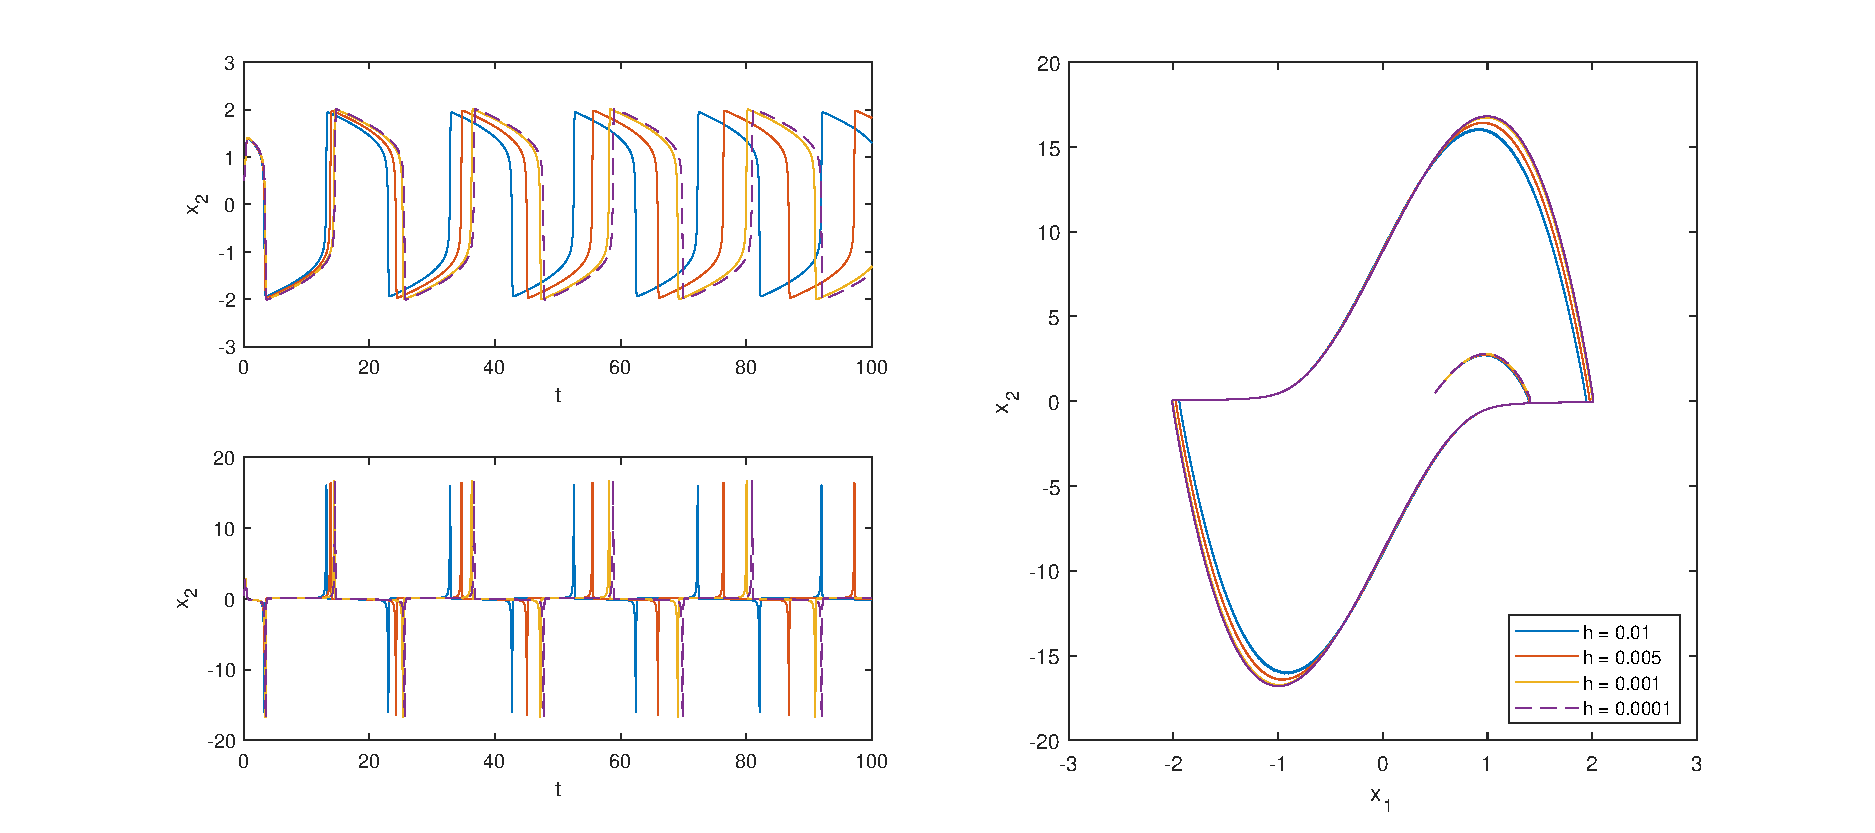
\includegraphics[width=1.25\textwidth]{images/3/3_4_fixed_mu_12.pdf}}
    \caption{Solution for the Van der Pol problem ($\mathit{\mu = 12}$) using Implicit Euler with fixed step size}
    \label{3_4_fixed_mu_12}
\end{figure}

\begin{figure}[H]
    \centering
    \makebox[\textwidth][c]{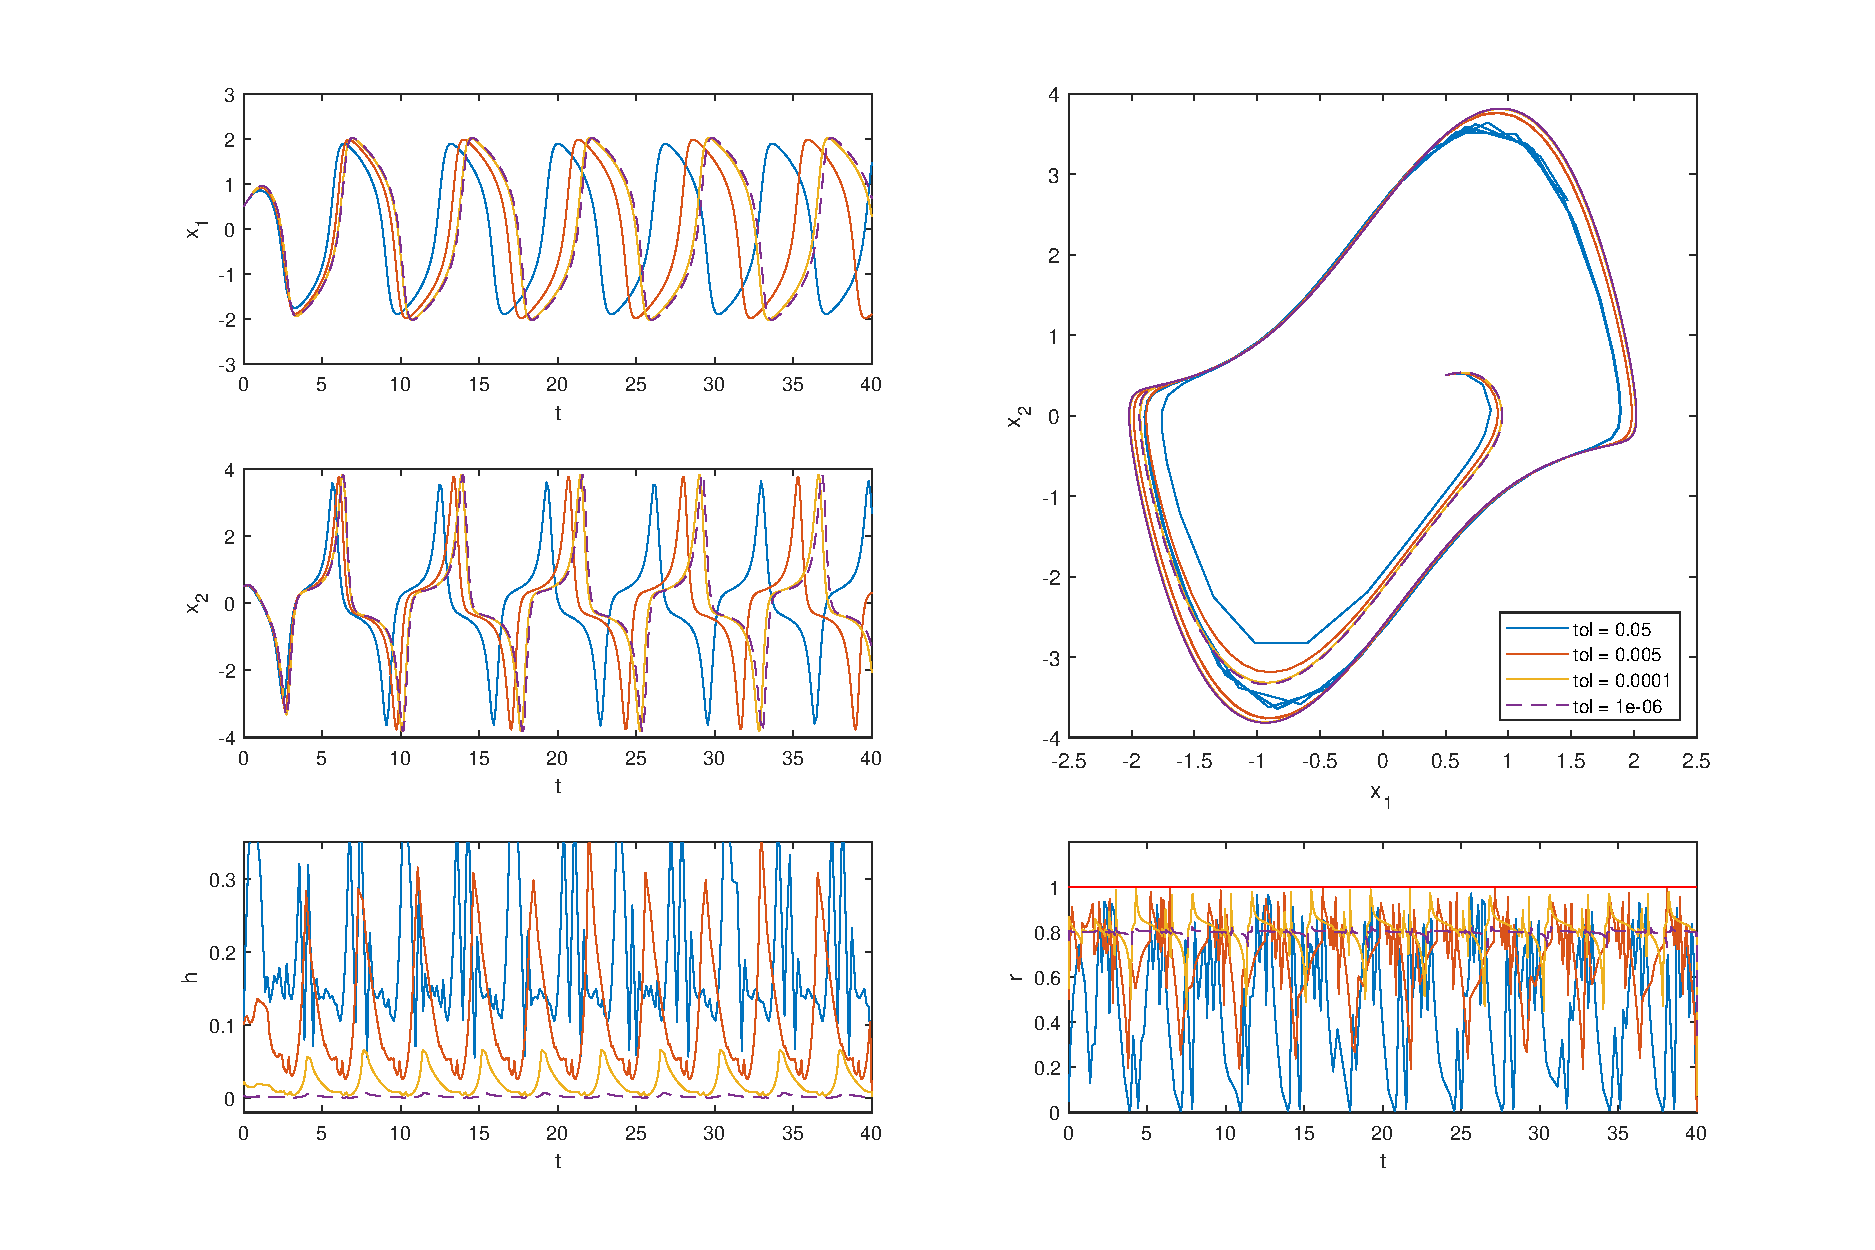
\includegraphics[width=1.25\textwidth]{images/3/3_4_adaptive_mu_2.pdf}}
    \caption{Solution for the Van der Pol problem ($\mathit{\mu = 2}$) using Implicit Euler with adaptive step size}
    \label{3_4_adaptive_mu_2}
\end{figure}

\begin{table}[H]
    \centering
    \begin{tabular}{@{}l|cccc@{}}
    \toprule
    Tolerances           & 0.05 & 0.005 & 0.0001 & 1e-06      \\ \midrule
    Function evaluations & 5732 & 8162  & 30764  & 3.0379e+05 \\
    Calculated steps     & 353  & 754   & 3799   & 37974      \\
    Accepted steps       & 237  & 589   & 3797   & 37972      \\
    Rejected steps       & 116  & 165   & 2      & 2          \\ \bottomrule
    \end{tabular}
    \caption{Parameters of the Implicit Euler with adaptive step size for the Van der Pol problem ($\mathit{\mu = 2}$)}
    \label{3_4_adaptive_mu_2_table}
\end{table}

\begin{figure}[H]
    \centering
    \makebox[\textwidth][c]{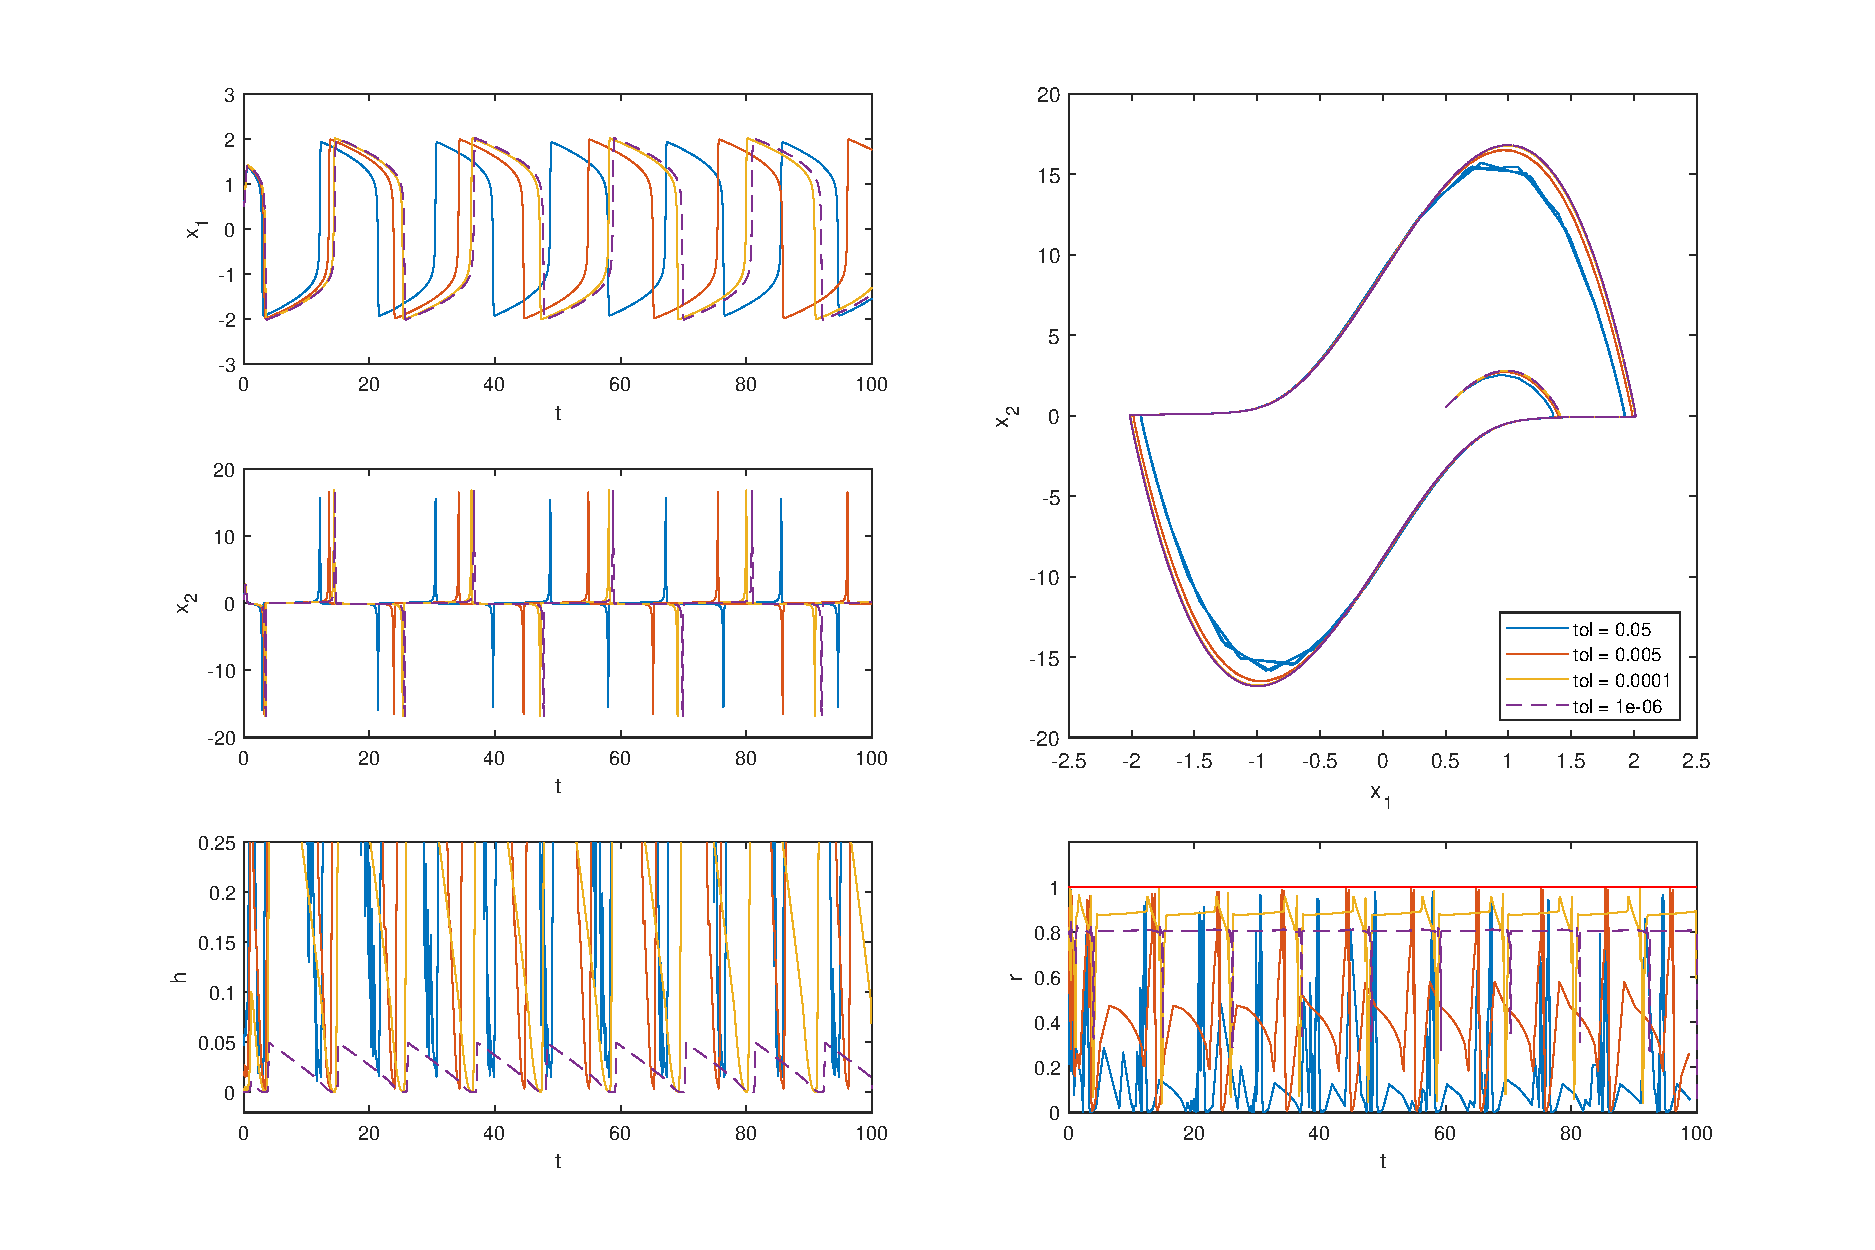
\includegraphics[width=1.25\textwidth]{images/3/3_4_adaptive_mu_12.pdf}}
    \caption{Solution for the Van der Pol problem ($\mathit{\mu = 12}$) using Implicit Euler with adaptive step size}
    \label{3_4_adaptive_mu_12}
\end{figure}

\begin{table}[H]
    \centering
    \begin{tabular}{@{}l|cccc@{}}    \toprule
    Tolerances           & 0.05  & 0.005 & 0.0001 & 1e-06      \\ \midrule
    Function evaluations & 24307 & 14368 & 48124  & 4.6157e+05 \\
    Calculated steps     & 776   & 1288  & 5746   & 57695      \\
    Accepted steps       & 478   & 982   & 5739   & 57692      \\
    Rejected steps       & 298   & 306   & 7      & 3          \\ \bottomrule
    \end{tabular}
    \caption{Parameters of the Implicit Euler with adaptive step size for the Van der Pol problem ($\mathit{\mu = 12}$)}
    \label{3_4_adaptive_mu_12_table}
\end{table}

\pagebreak
%%%%%%%%%%%%%%%%%%%%%%%%%%%%%%%%%%%%%%%%%%%%%%%%%%%%%%%%%%%%%%%%%%%%%%%%%%%%%%%%%%%%%%%%%%%%%%%%%%%

\subsection{Test  your  algorithms  on  the  adiabatic  CSTR  problem  described  in  the
papers uploaded to Learn (3D-version and 1D-version).}
Here are shown the results of the Implicit Euler for the CSTR problem. Just as in last exercise, we can't observe any significant difference between the 3D and 1D problem (Figure \ref{3_5_3D_vs_1D}). The results when working with a fixed time step size (Figure \ref{3_5_3D_1D_hs}) are the same for both results. We can observe how the implicit manages to control the \textit{stiffness} of the problem when the values of $F$ go lower, we can't find no longer the oscillations. The highest step size misses completely the values though. However, it converges quicker than the explicit to the real solution.

For the adaptive method, the value \code{facmax} was set to be $1.5$, otherwise the asymptotic step controller was too sensible and diverged a lot. Here, we can see that the step size controller is working and the results converge quickly to the real solution. The 1D solution misses the larger values of $T$ (when $F$ is lower) for the largest tolerance. 
\begin{figure}[H]
    \centering
    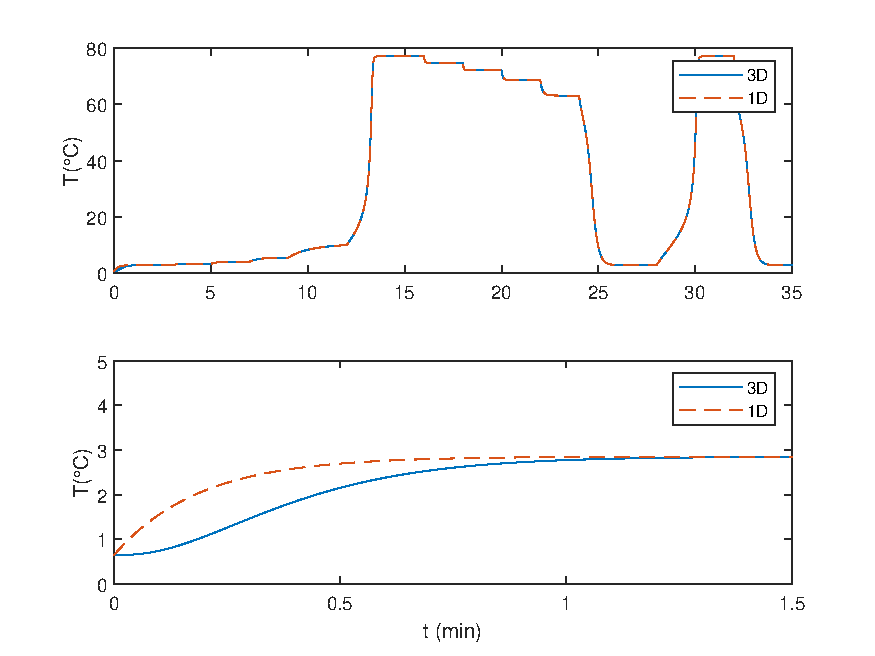
\includegraphics[width=0.8\textwidth]{images/3/3_5_3D_vs_1D.pdf}
    \caption{Comparison of the solutions for the CSTR 3D and 1D with Implicit Euler}
    \label{3_5_3D_vs_1D}
\end{figure}

\begin{figure}[H]
\centering
    \begin{subfigure}{0.8\linewidth}
        \centering
        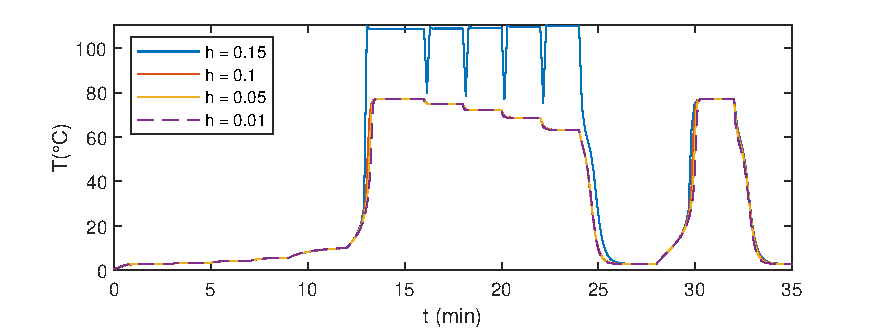
\includegraphics[width=1\linewidth]{images/3/3_5_3D_hs.pdf} 
        \caption{CSTR 3D problem}
    \end{subfigure} \\
    \begin{subfigure}{0.8\linewidth}
        \centering
        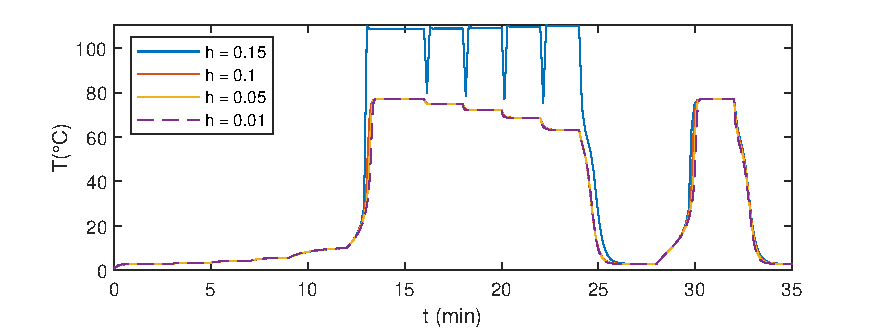
\includegraphics[width=1\linewidth]{images/3/3_5_1D_hs.pdf}
        \caption{CSTR 1D problem}
    \end{subfigure}
    \caption{Solution for the CSTR problem using Implicit Euler with fixed step size}
    \label{3_5_3D_1D_hs}
\end{figure}

\begin{figure}[H]
    \centering
    \makebox[\textwidth][c]{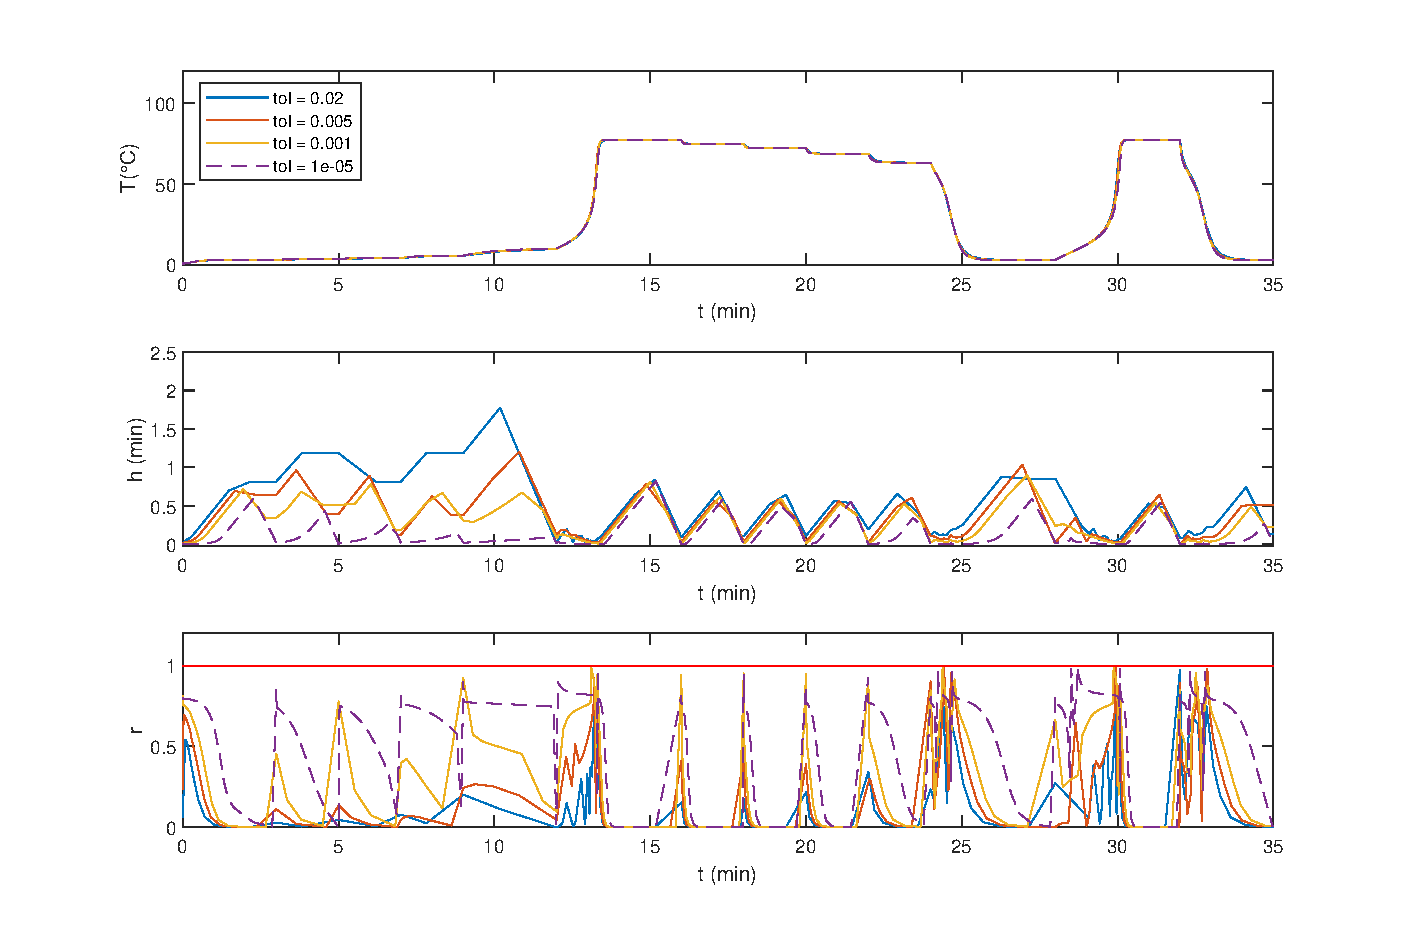
\includegraphics[width=1\textwidth]{images/3/3_5_3D_tols.pdf}}
    \caption{Solution for the CSTR 3D problem using Implicit Euler with adaptive step size}
    \label{3_5_3D_tols}
\end{figure}

\begin{table}[H]
    \centering
    \begin{tabular}{@{}l|cccc@{}}
    \toprule
    Tolerances           & 0.02 & 0.005 & 0.001 & 1e-05 \\ \midrule
    Function evaluations & 2386 & 3171  & 4325  & 21476 \\
    Calculated steps     & 146  & 232   & 388   & 2589  \\
    Accepted steps       & 121  & 188   & 307   & 2537  \\
    Rejected steps       & 25   & 44    & 81    & 52    \\ \bottomrule
    \end{tabular}
    \caption{Parameters of the Implicit Euler with adaptive step size for the CSTR 3D problem}
    \label{3_5_3D_tols_table}
\end{table}

\begin{figure}[H]
    \centering
    \makebox[\textwidth][c]{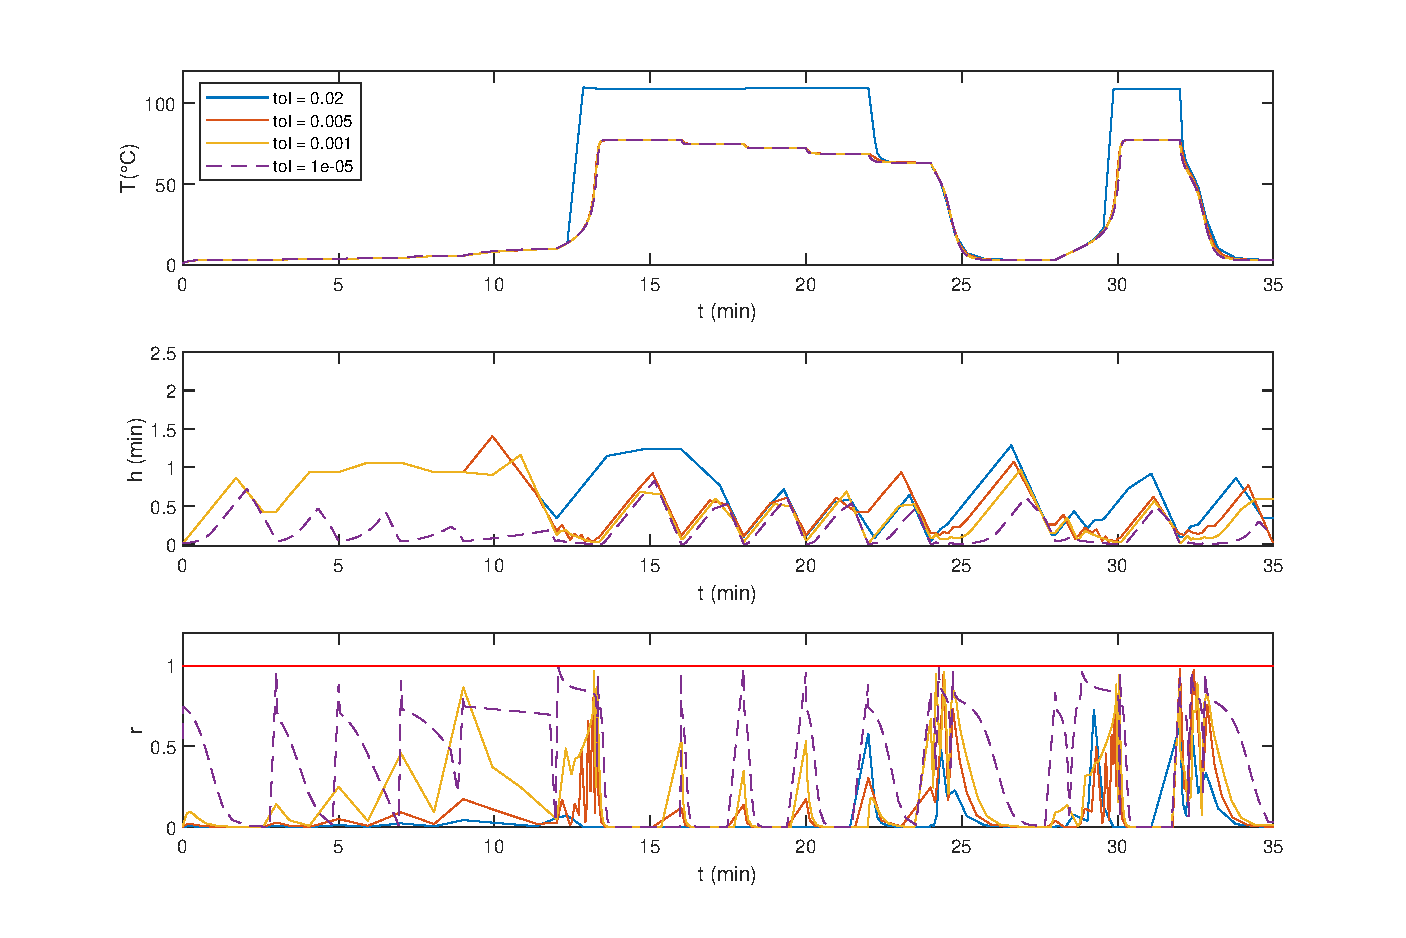
\includegraphics[width=1\textwidth]{images/3/3_5_1D_tols.pdf}}
    \caption{Solution for the CSTR 1D problem using Implicit Euler with adaptive step size}
    \label{3_5_1D_tols}
\end{figure}

\begin{table}[H]
    \centering
    \begin{tabular}{@{}l|cccc@{}}
    \toprule
    Tolerances           & 0.02 & 0.005 & 0.001 & 1e-05 \\ \midrule
    Function evaluations & 2311 & 2592  & 3144  & 11390 \\
    Calculated steps     & 88   & 141   & 222   & 1126  \\
    Accepted steps       & 80   & 115   & 173   & 1073  \\
    Rejected steps       & 8    & 26    & 49    & 53    \\ \bottomrule
    \end{tabular}
    \caption{Parameters of the Implicit Euler with adaptive step size for the CSTR 1D problem}
    \label{3_5_1D_tols_table}
\end{table}

%%%%%%%%%%%%%%%%%%%%%%%%%%%%%%%%%%%%%%%%%%%%%%%%%%%%%%%%%%%%%%%%%%%%%%%%%%%%%%%%%%%%%%%%%%%%%%%%%%%

\subsection{Compare the results from your algorithms with the results you get using some  of  Matlab's  ODE  solvers  The  report  should  contain  figures  and  a discussion of your algorithm for different tolerances and step sizes.}
For the Van der Pol problem, we tested Implicit Euler against \code{ode45} for the non-stiff case ($\mu = 1.5$), and against \code{ode15s} for the stiff case ($\mu = 15$). Contrary to what we obtained using explicit Euler, the Implicit Euler works fine in the stiff case, even though the \code{ode15s} achieves better accuracy with a fewer no. of function evaluations. This is also due to the fact that we're using step doubling to approximate the error. In the non-stiff case, however, the no. of evaluations is ridiculously high compared to the \code{ode45}, which makes sense given that it's an implicit method vs. an explicit one in a non-stiff problem.

\begin{figure}[H]
    \centering
    \makebox[\textwidth][c]{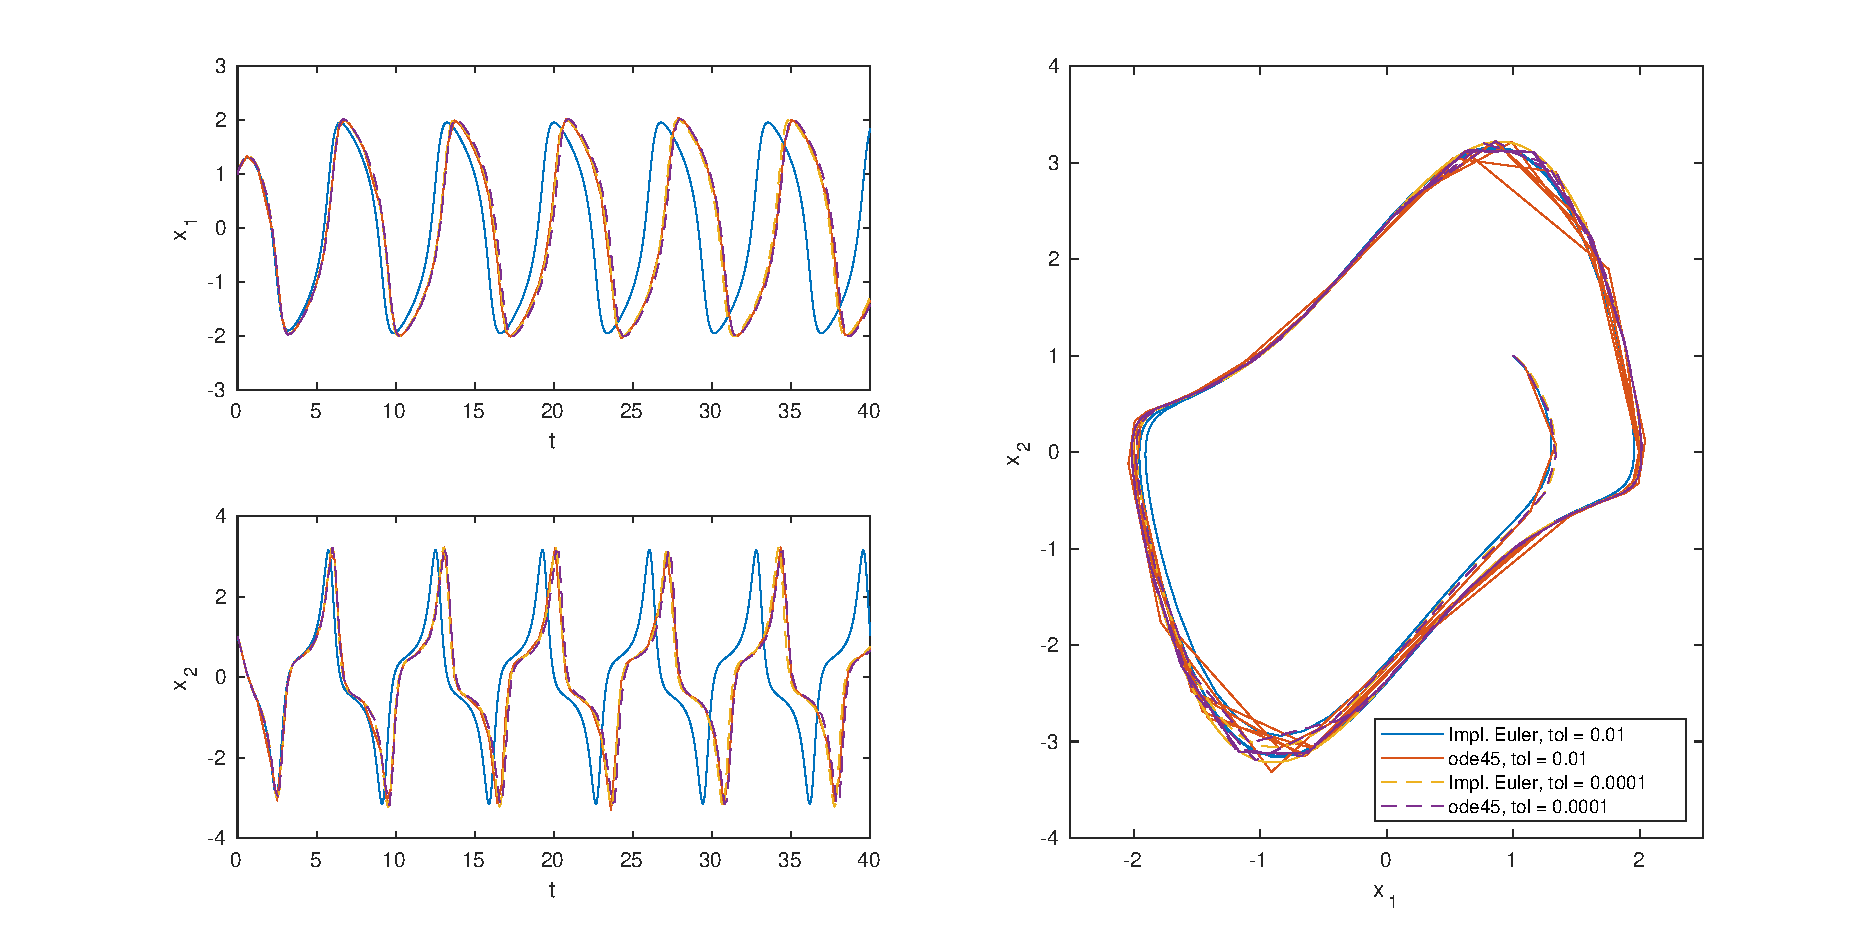
\includegraphics[width=1.25\textwidth]{images/3/3_6_mu_1_5.pdf}}
    \caption{Solution for the Van der Pol problem ($\mathit{\mu = 1.5}$) using Implicit Euler vs. \code{ode45}}
    \label{3_6_mu_1_5}
\end{figure}

\begin{table}[H]
    \centering
    \begin{tabular}{@{}l|cc|cc@{}}
    \toprule
    \textbf{Method}      & \multicolumn{2}{c|}{\textbf{Impl. Euler}} & \multicolumn{2}{c}{\textbf{ode45}} \\
    Tolerances           & 0.01               & 0.0001               & 0.01            & 0.0001           \\ \midrule
    Function evaluations & 5713               & 29600                & 787             & 1357             \\
    Calculated steps     & 522                & 3666                 & 131             & 226              \\
    Accepted steps       & 402                & 3664                 & 100             & 180              \\
    Rejected steps       & 120                & 2                    & 31              & 46               \\ \bottomrule
    \end{tabular}
    \caption{Parameters of the Implicit Euler vs. \code{ode45} for the Van der Pol problem ($\mathit{\mu = 1.5}$)}
    \label{3_6_adaptive_mu_1_5_table}
\end{table}

\begin{figure}[H]
    \centering
    \makebox[\textwidth][c]{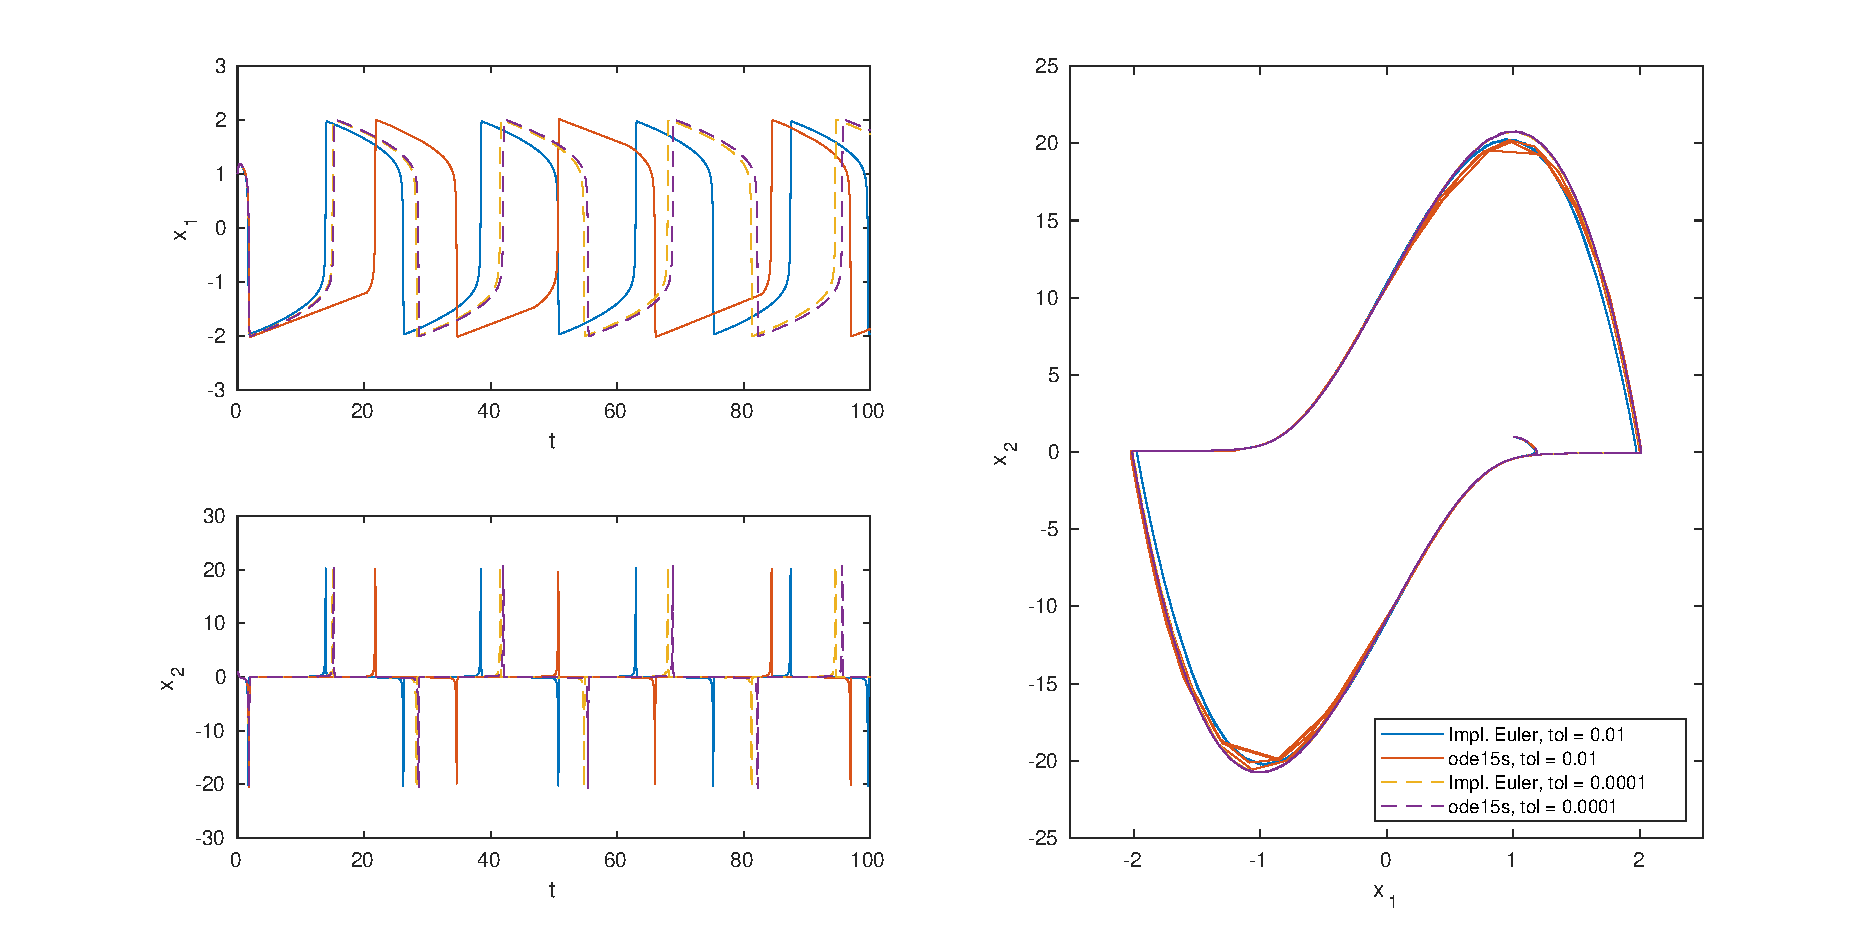
\includegraphics[width=1.25\textwidth]{images/3/3_6_mu_15.pdf}}
    \caption{Solution for the Van der Pol problem ($\mathit{\mu = 15}$) using Implicit Euler vs. \code{ode15s}}
    \label{3_6_mu_15}
\end{figure}

\begin{table}[H]
    \centering
    \begin{tabular}{@{}l|ll|ll@{}}
    \toprule
    \textbf{Method}      & \multicolumn{2}{c|}{\textbf{Impl. Euler}} & \multicolumn{2}{c}{\textbf{ode15s}} \\
    Tolerances           & 0.01                & 0.0001              & 0.01            & 0.0001            \\ \midrule
    Function evaluations & 12508               & 43567               & 1273            & 2780              \\
    Calculated steps     & 937                 & 5198                & 558             & 1327              \\
    Accepted steps       & 743                 & 5189                & 411             & 1094              \\
    Rejected steps       & 120                 & 2                   & 147             & 233               \\ \bottomrule
    \end{tabular}
    \caption{Parameters of the Implicit Euler vs. \code{ode15s} for the Van der Pol problem ($\mathit{\mu = 15}$)}
    \label{3_6_adaptive_mu_15_table}
\end{table}

For the CSTR problem, we also see how both the Implicit Euler and \code{ode15s} achieve good performance for the 3D case. For the 1D case we see the Implicit deviating a bit, but this could be caused by the tolerance being too wide. The \code{ode45} achieves worse performance in both cases.

\begin{figure}[H]
    \centering
    \begin{subfigure}{0.8\linewidth}
        \centering
        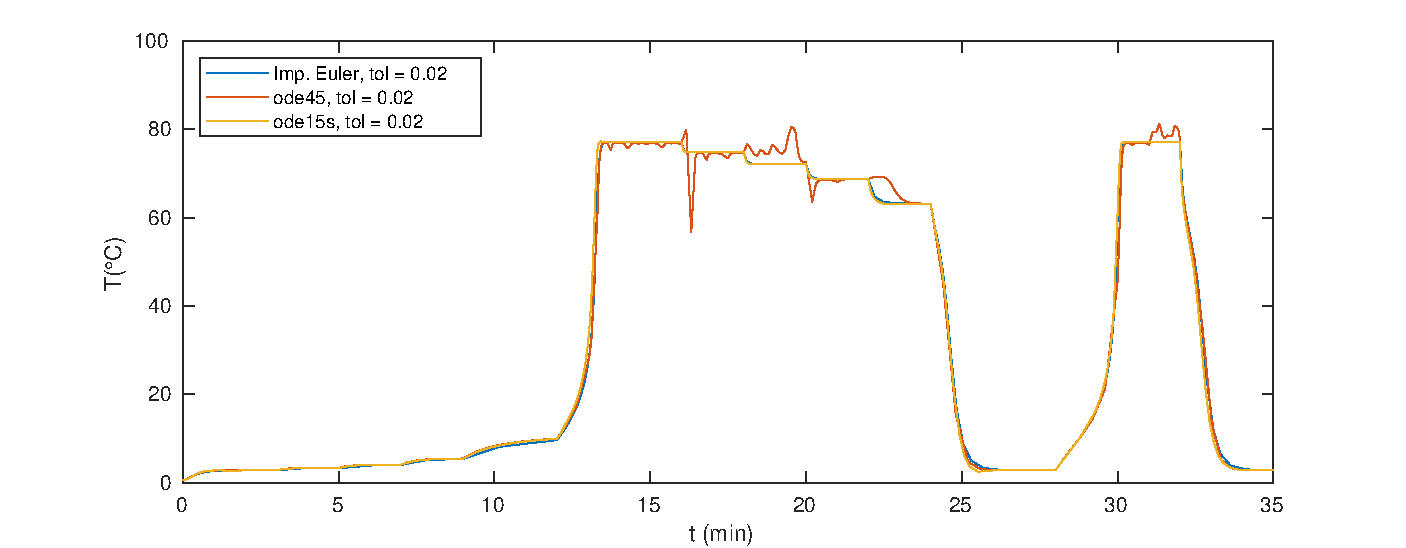
\includegraphics[width=1\linewidth]{images/3/3_6_3D.pdf} 
        \caption{CSTR 3D problem}
    \end{subfigure} \\
    \begin{subfigure}{0.8\linewidth}
        \centering
        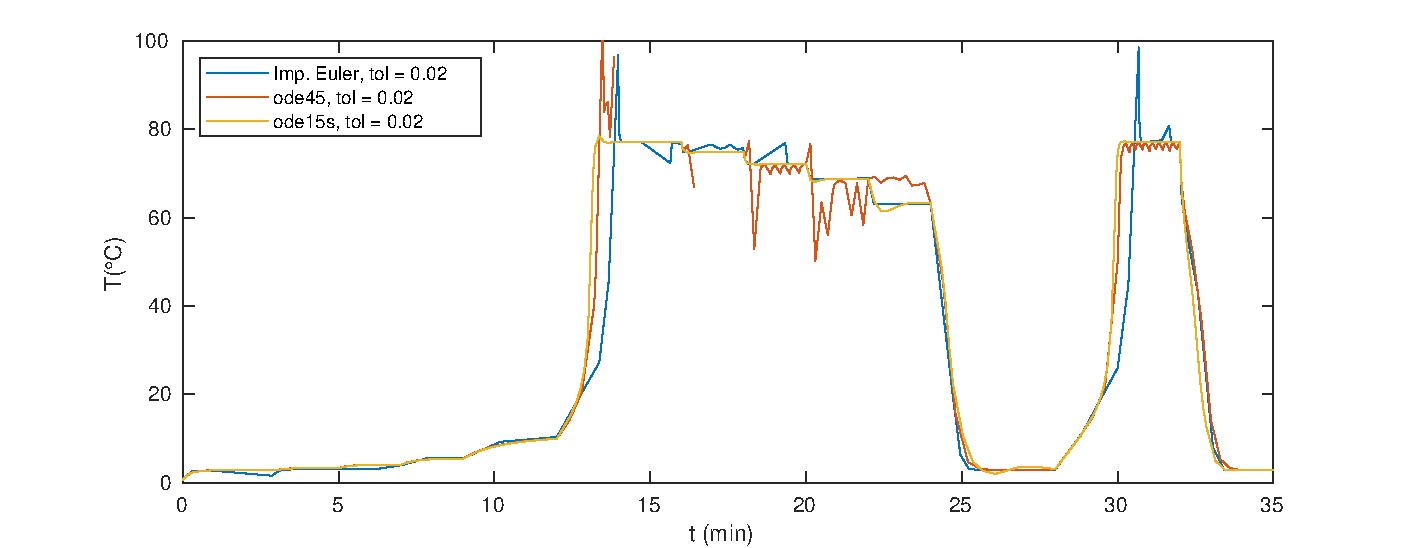
\includegraphics[width=1\linewidth]{images/3/3_6_1D.pdf}
        \caption{CSTR 1D problem}
    \end{subfigure}
    \caption{Solution for the CSTR problem using Implicit Euler vs. \code{ode45} and \code{ode15s}}
    \label{3_6_3D_1D}
\end{figure}

\begin{table}[H]
    \centering
    \begin{tabular}{@{}l|c|c|c@{}}
    \toprule
    \textbf{Method}      & \textbf{Impl. Euler} & \textbf{ode45} & \textbf{ode15s} \\
    Tolerances           & 0.02                 & 0.02           & 0.02            \\ \midrule
    Function evaluations & 2386                 & 1513           & 477             \\
    Calculated steps     & 146                  & 1586           & 1408            \\
    Accepted steps       & 121                  & 220            & 201             \\
    Rejected steps       & 25                   & 30             & 29              \\ \bottomrule
    \end{tabular}
    \caption{Parameters of the Implicit Euler vs. \code{ode45} and \code{ode15s} for the CSTR-3D problem}
    \label{3_6_3D_table}
\end{table}

\begin{table}[H]
    \centering
    \begin{tabular}{@{}l|c|c|c@{}}
    \toprule
    \textbf{Method}      & \textbf{Impl. Euler} & \textbf{ode45} & \textbf{ode15s} \\
    Tolerances           & 0.02                 & 0.02           & 0.02            \\ \midrule
    Function evaluations & 201                  & 1297           & 375             \\
    Calculated steps     & 117                  & 1270           & 1275            \\
    Accepted steps       & 84                   & 195            & 180             \\
    Rejected steps       & 33                   & 19             & 27              \\ \bottomrule
    \end{tabular}
    \caption{Parameters of the Implicit Euler vs. \code{ode45} and \code{ode15s} for the CSTR-1D problem}
    \label{3_6_1D_table}
\end{table}

\pagebreak
%%%%%%%%%%%%%%%%%%%%%%%%%%%%%%%%%%%%%%%%%%%%%%%%%%%%%%%%%%%%%%%%%%%%%%%%%%%%%%%%%%%%%%%%%%%%%%%%%%%

\subsection{Discuss when one should use the implicit Euler method rather than the
explicit Euler method and illustrate that using an example.}
As previously discussed, the Implicit Euler method is a lot more robust than the Explicit, this is, it handles \textit{stiff problems} a lot better. The reason behind this behaviour is connected to the \textit{region of stability} of the method. We showed the region of stability for the Explicit and Implicit Euler in Figure \ref{stability_regions}. The problem can require an extremely low $h$ for the Explicit Method in order to satisfy $|y_{n-1}| \leq |y_n|$. The implicit, being A-stable, doesn't have this problem.

If we solve the Van der Pol problem for $\mu = 100$ with Explicit and Implicit method with adaptive step we will observe this behaviour. Both will be solved with a tolerance of $10^{-3}$. Just by looking at the $h$ vs. time and $r$ vs. time we can notice the difference. Notice that the time step with the Explicit must be really small even though the solution is really smooth. Otherwise, it would explode. The Implicit manages the stiffness a lot better, getting to values of time step of more than $8$ units of time. The solution is equally valid in both of them. Looking at table \ref{3_7_table}, we notice that the number of steps calculated is more than $10$ times smaller on the implicit. In this case, the Implicit proves to be computationally better, even though we are calling the Newton method at every time step. 

\begin{figure}[H]
    \centering
    \makebox[\textwidth][c]{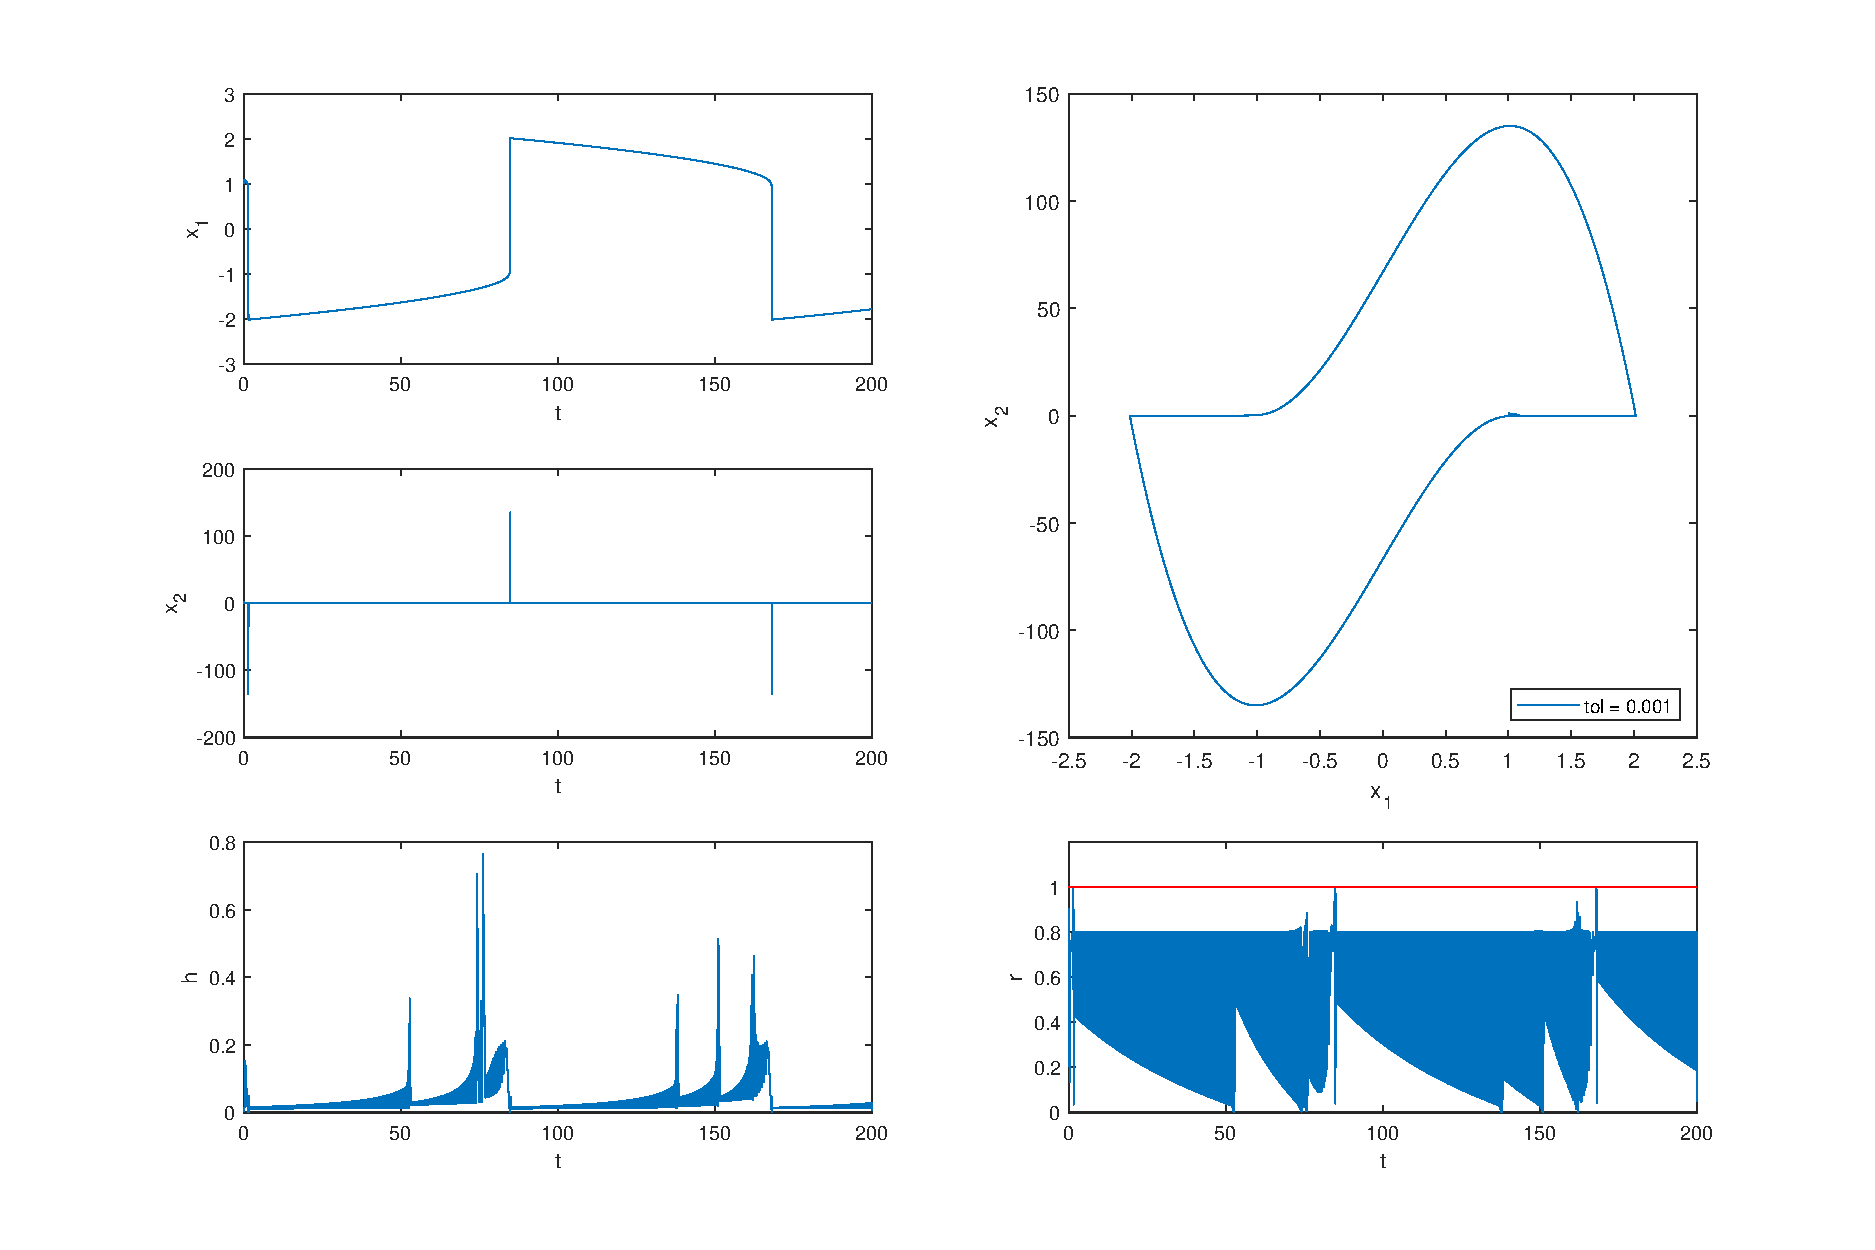
\includegraphics[width=1.25\textwidth]{images/3/3_7_explicit.pdf}}
    \caption{Solution for the Van der Pol problem ($\mathit{\mu = 100}$) using Explicit Euler with adaptive step size}
    \label{3_7_explicit}
\end{figure}

\begin{figure}[H]
    \centering
    \makebox[\textwidth][c]{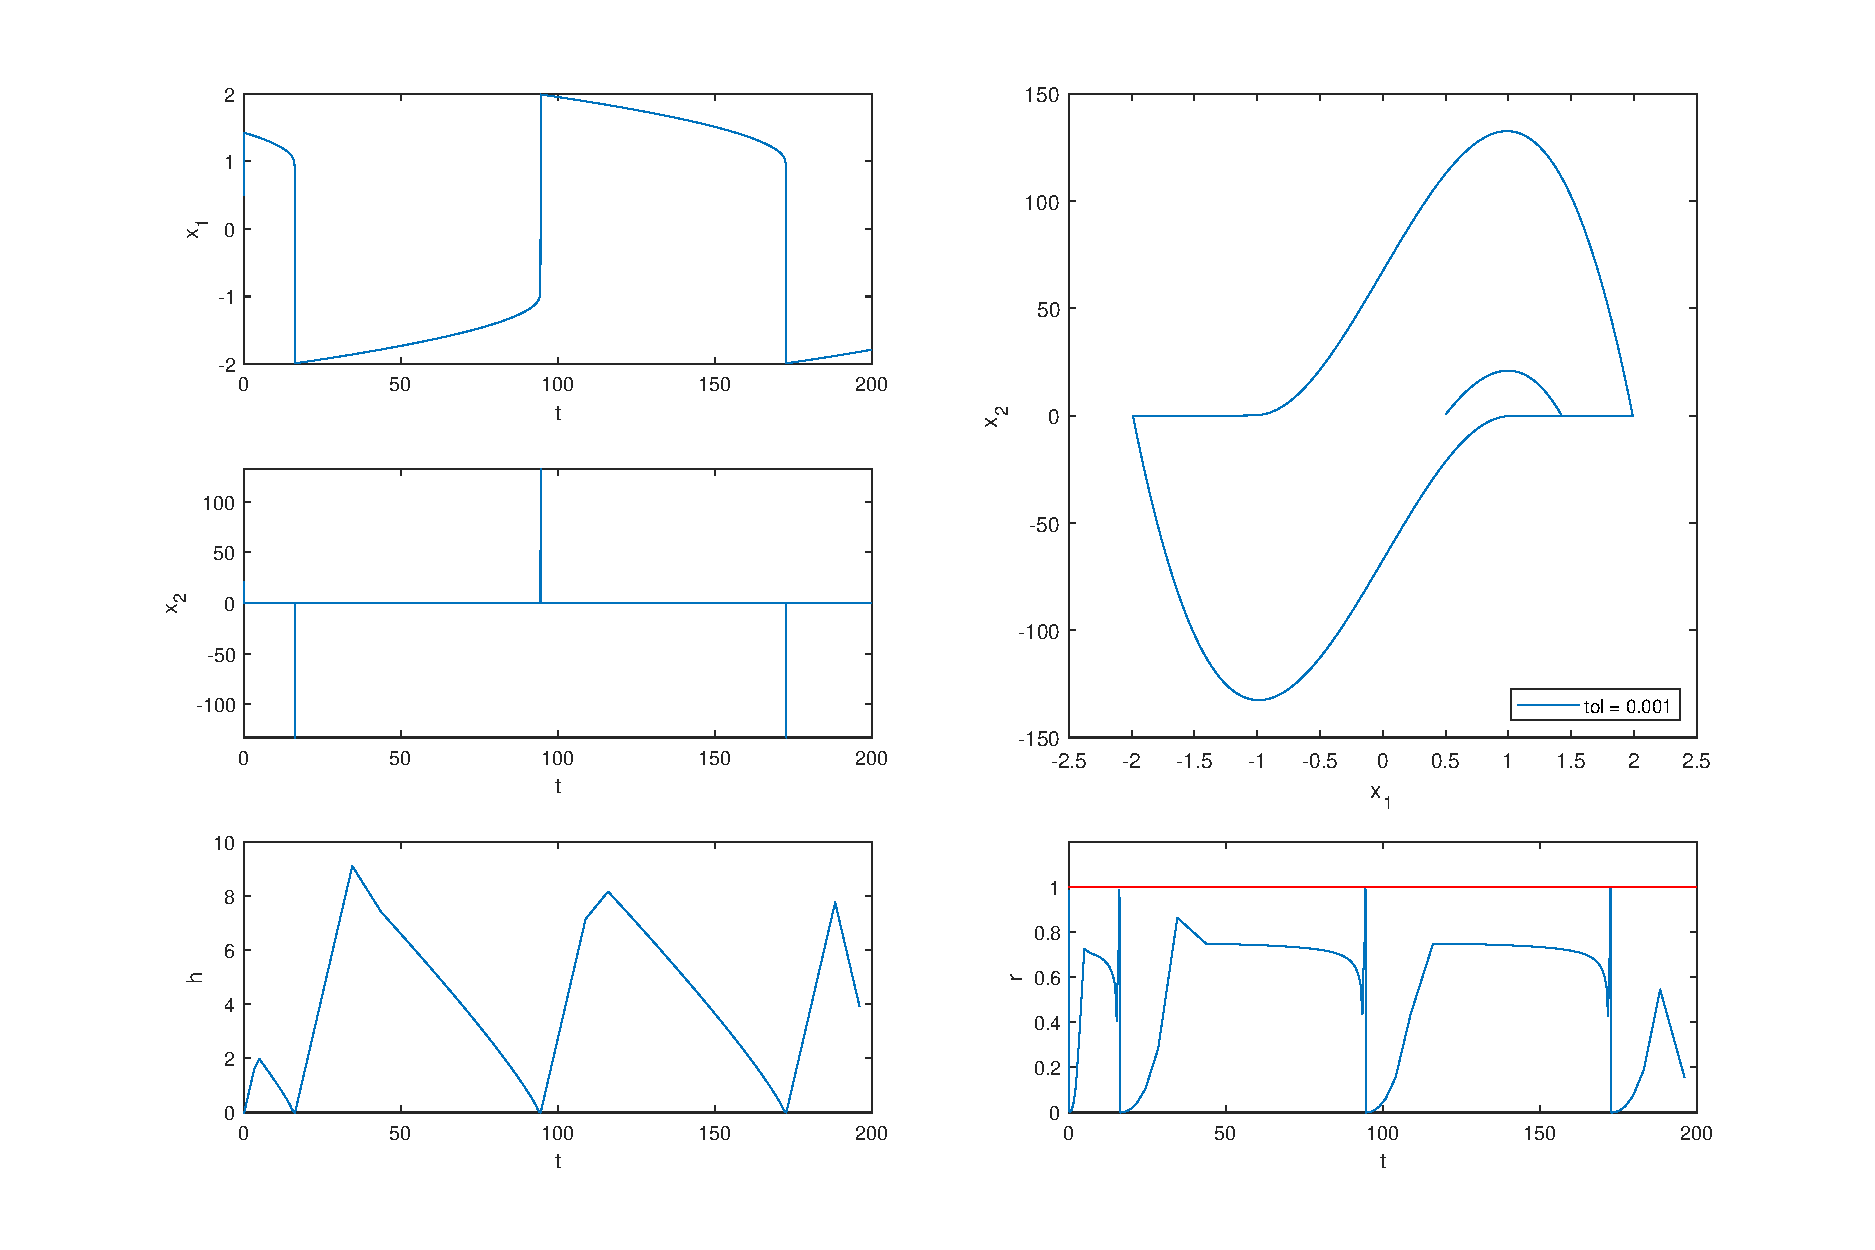
\includegraphics[width=1.25\textwidth]{images/3/3_7_implicit.pdf}}
    \caption{Solution for the Van der Pol problem ($\mathit{\mu = 100}$) using Implicit Euler with adaptive step size}
    \label{3_7_implicit}
\end{figure}

\begin{table}[H]
\centering
\begin{tabular}{@{}l|cc@{}}
\toprule
Tolerances           & Explicit & Implicit \\ \midrule
Function evaluations & 22654    & 12407    \\
Calculated steps     & 13450    & 1207     \\
Accepted steps       & 9204     & 1076     \\
Rejected steps       & 4246     & 131      \\ \bottomrule
\end{tabular}
\caption{Parameters of the Explicit and Implicit methods for the Van der Pol problem ($\mu = 100$)}
\label{3_7_table}
\end{table}